
\section{Bug Localization}
\begin{figure}[H]
\centering
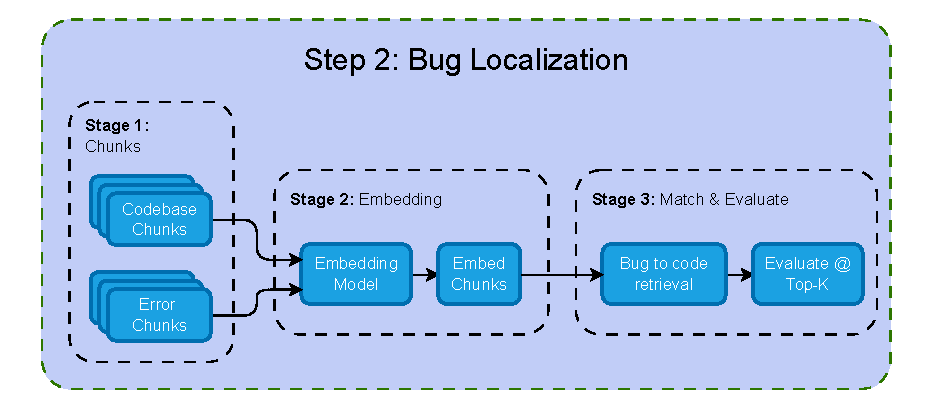
\includegraphics[width=1\columnwidth]{Figures/Step2_bug_localization.drawio.pdf}
\caption{Bug localization pipeline}
\label{fig:step2_bug_localization}
\end{figure}

\subsection{Model Selection and Performance}
Empirically, we find that smaller models trained specifically on code embeddings outperform both general-purpose language models and larger code models in our localization task. Table~\ref{tab:model_performance_at_k} summarizes the top-$k$ accuracy across several embedding models. We adopt the \texttt{blaze} model due to its strong performance and efficient resource usage; It supports batch sizes up to 128 on an 8GB GPU, compared to over 15GB required by larger models such as \texttt{jinaai/jina-embedding-v2-base-code} at batch size 2. Earlier experiments with \texttt{MiniLM-L12-v2} served as a baseline, yielding 60\% Top-5 accuracy.

\subsection{Retrieval Method}
For retrieval, we compute cosine similarity between the embedded bug trace and each code chunk, returning the top-$k$ most similar candidates. As shown in Figure~\ref{fig:blaze@k_graph}, performance improves significantly between $k=1$ and $k=10$.

\subsection{Dataset Characteristics}
We also observe that localization accuracy declines in projects with larger file counts. Table~\ref{tab:bugsinpy_projects} highlights that \texttt{pandas}, \texttt{matplotlib}, \texttt{ansible}, and \texttt{youtube-dl} have substantially larger codebases, and three of the four have reduced performance compared to other projects. This suggests that increasing the search space negatively impacts retrieval precision, even when using semantically rich embeddings.
\subsection{Evaluation Bias}
Table~\ref{fig:blaze@k_graph_file} presents top-$k$ accuracy based on the file name, while Table\ref{fig:blaze@k_graph_function} reports performance based on the function name.

\begin{figure}[H]
\centering
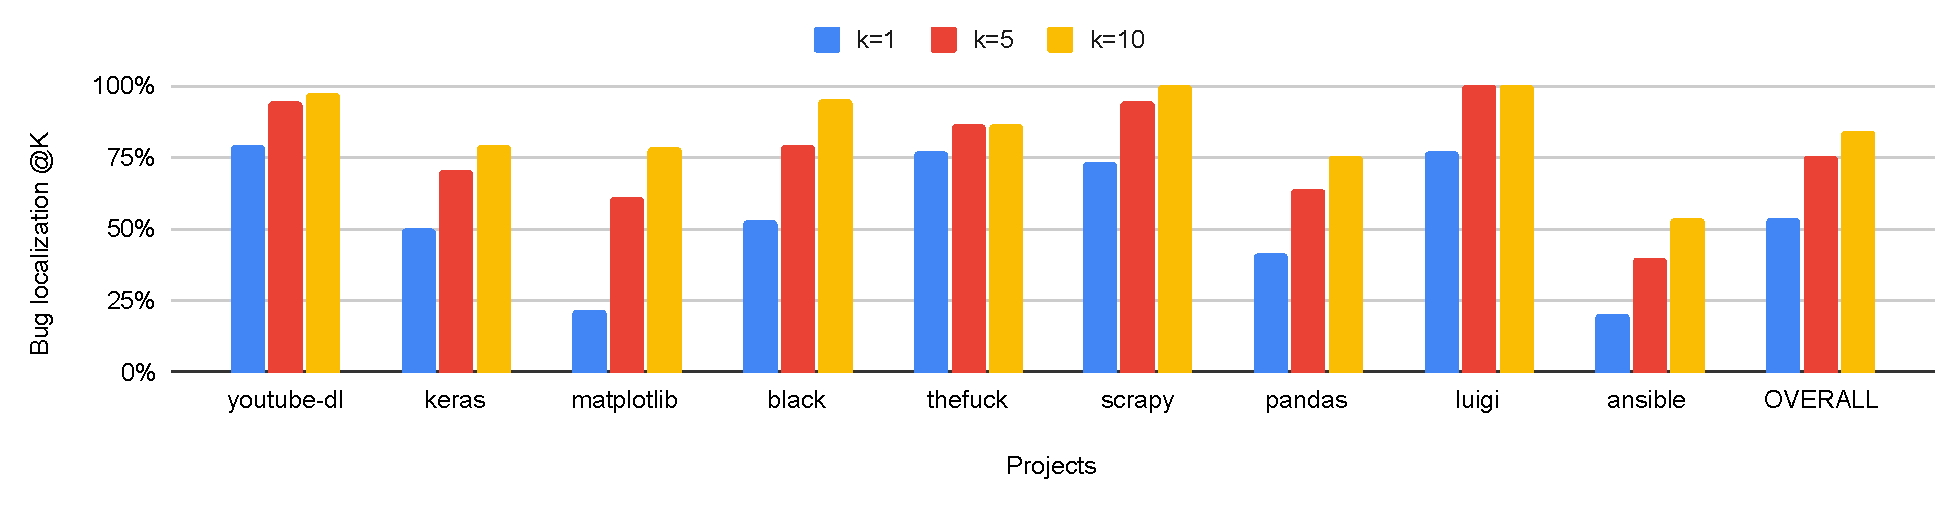
\includegraphics[width=1\columnwidth]{Figures/blaze@k_file.pdf}
\caption{File level bug localization accuracy @k for "blaze" a fine-tuned version of "codesage/codesage\_small\_v2"}
\label{fig:blaze@k_graph_file}
\end{figure}

\begin{figure}[H]
\centering
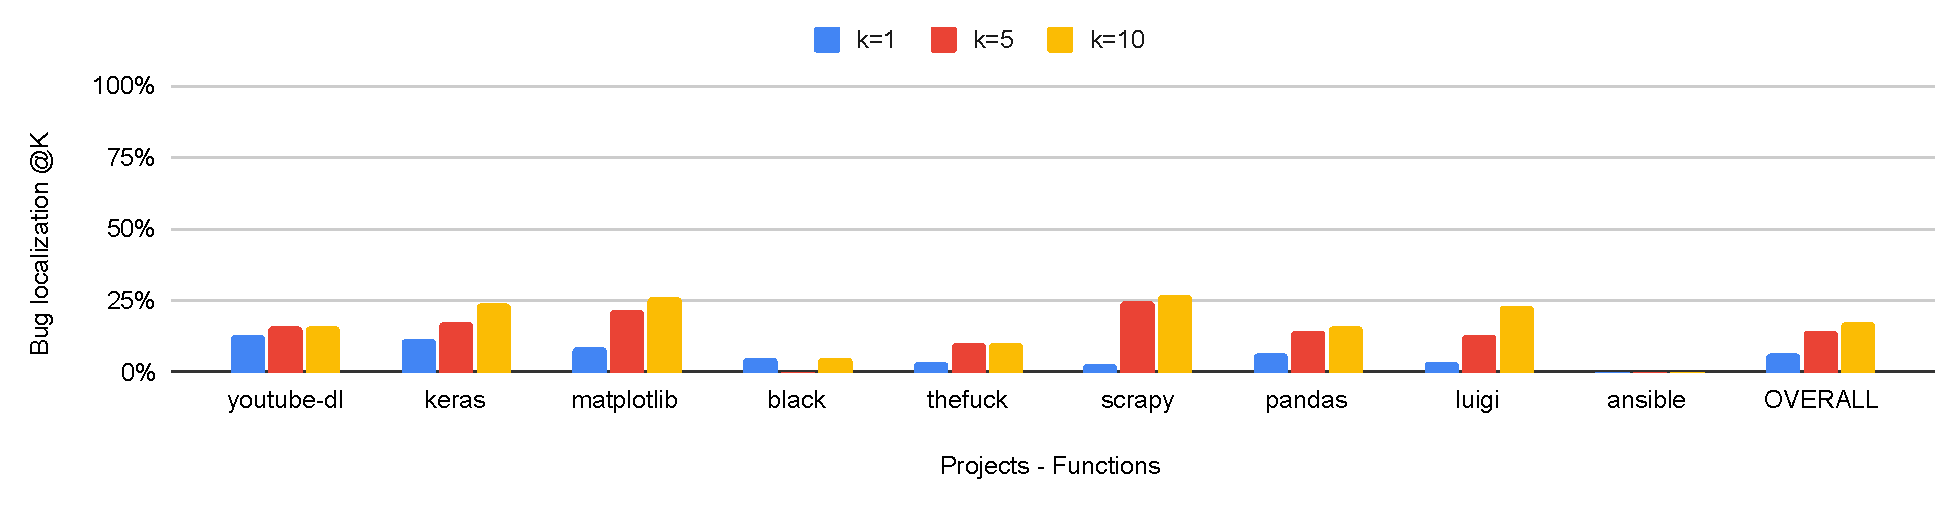
\includegraphics[width=1\columnwidth]{Figures/blaze@k_function.pdf}
\caption{Function level bug localization accuracy @k for "blaze" a fine-tuned version of "codesage/codesage\_small\_v2"}
\label{fig:blaze@k_graph_function}
\end{figure}

\begin{table}[H]
\centering
\begin{tabularx}{\textwidth}{lccccc}
\toprule
\textbf{Model} & \textbf{Top-1} & \textbf{Top-5} & \textbf{Top-10} & \textbf{MAP@60} & \textbf{MRR@60} \\
\midrule
BLAZE & 53.76\% & 75.43\% & 84.10\% & 40.81\% & 63.91\% \\
all-MiniLM-L12-v2 & 39.94\% & 63.85\% & 72.89\% & 32.15\% & 51.11\% \\
\bottomrule
\end{tabularx}
\caption{Overall success rate @k for different models at the file level}
\label{tab:model_performance_at_k}
\end{table}


\begin{table}[H]
\centering
\begin{tabularx}{\textwidth}{lccccc}
\toprule
\textbf{Model} & \textbf{Top-1} & \textbf{Top-5} & \textbf{Top-10} & \textbf{MAP@60} & \textbf{MRR@60} \\
\midrule
BLAZE & ?\% & ?\% & ?\% & ?\% & ?\% \\
\bottomrule
\end{tabularx}
\caption{Overall success rate @k for different models at the function level}
\label{tab:model_performance_at_k}
\end{table}
